
%(BEGIN_QUESTION)
% Copyright 2013, Tony R. Kuphaldt, released under the Creative Commons Attribution License (v 1.0)
% This means you may do almost anything with this work of mine, so long as you give me proper credit

Calculate the necessary value for resistor $R_2$ in this circuit to provide an output voltage ($V_{out}$) of 5.8 volts:

$$\includegraphics[width=15.5cm]{i02071x01.eps}$$

$R_2$ = 

\vskip 10pt

Also, mark the polarity of $V_{out}$ with ``+'' and ``$-$'' symbols.

\vskip 10pt

\underbar{file i02071}
%(END_QUESTION)





%(BEGIN_ANSWER)

$R_2$ = 2.711 k$\Omega$

\vskip 10pt

$V_{out}$ is positive on the right and negative on the left.

%(END_ANSWER)





%(BEGIN_NOTES)

{\bf This question is intended for exams only and not worksheets!}.

%(END_NOTES)

